\documentclass[12pt]{article}

\usepackage{sbc-template}
\usepackage[utf8]{inputenc}
\usepackage{graphicx,url}
\usepackage[pdftex]{hyperref}

\usepackage[brazil]{babel}   
%\usepackage[latin1]{inputenc}  

     
\sloppy


\title{Gerando códigos para melhoria do Teste Funcional Automatizado de ferramentas de Gerenciamento de Processos de Negócio}
%Uma estratégia para geração de códigos para Teste Funcional de ferramentas de Gerenciamento de Processos de Negócio

\author{Jéssica Lasch de Moura\inst{1}, Andrea Schwertner Charão\inst{1}}

\address{Centro de Tecnologia -- Universidade Federal de Santa Maria
  (UFSM)\\
  Santa Maria -- RS -- Brazil
\nextinstitute
  Laboratório de Sistemas de Computação (LSC) -- Universidade Federal de Santa Maria\\  
  \email{\{jmoura,andrea\}@inf.ufsm.br}
}
\begin{document} 

\maketitle

\begin{abstract}
This paper describes a strategy created to get artifacts used in the implementation of automated functional testing of Business Process Management tools. The objective of this work was to facilitate the tests and improve the scope of the same, in order to improve the applications in question. With this strategy, it was possible to obtain important information about the processes and generate important elements for functional testing, making it the fastest and most complete test case.
\end{abstract}
     
\begin{resumo} 
Este trabalho descreve um estratégia criada para obter artefatos utilizados na execução de testes funcionais automatizados de ferramentas de Gestão de Processos de Negócio. O objetivo deste trabalho era facilitar a execução dos testes bem como melhorar a abrangência dos mesmos, visando a melhoria das aplicações em questão. Com esta estratégia, foi possível obter informações importantes sobre os processos e gerar elementos importantes para o teste funcional, tornando a etapa de teste mais rápida e completa.
\end{resumo}

\section{Introdução}

 \begin{itemize}
   \item BPM
   \item Teste com BPM pouco abordado + importância dos testes;
   \item Citar trabalho anterior (abordagem utilizadas para ferramentas web em geral)= teste com selenium e cucumber se mostrou mais promissor;
   \begin{itemize}
	\item Pode ser trabalhoso criar os elementos necessários para o teste completo;
   \end{itemize}
   \item Para melhoria na criação dos testes: analisar o diagrama no formato BPMN, através do parser criado, para gerar informações
     \begin{itemize}
	\item Facilitar/tornar mais rápida a criação dos elementos
	\item Aumento na cobertura dos testes (cria todos cenários possíveis)
   \end{itemize}
   \item Objetivo:  melhorar e facilitar o teste funcional automatizado de aplicações bpm;
 \end{itemize}
 
%Mesmo utilizando ferramentas para teste automatizado, alguns elementos necessários podem ter sua criação trabalhosa
%ainda assim, depende de algumas etapas, como a criação de casso de testes...
	
\section{BPM e Teste}
%-Teste funcional ajuda a aumentar a qualidade do software;
%-sistemas bpm = web, permite executar testes funcionais com ferramenta
%-Teste é pouco abordado
%-Teste é importante

O termo BPM pode ser usado com ênfases diferentes, às vezes com foco em tecnologia (software) e outras vezes em gestão. Mesmo assim, a área tem convergido no entendimento do ciclo de vida de aplicações de BPM, que envolve as atividades de análise, modelagem, execução, monitoramento e otimização~\cite{ABPMP}. 

Os sistemas de BPM (BPMS) têm se afirmado como ferramentas essenciais para suporte a atividades desse ciclo de vida. Atualmente, pode-se dizer que um típico BPMS oferece recursos para definição e modelagem de processos em BPMN, controle da execução e monitoramento de atividades dos processos~\cite{forrester}. Há uma tendência dos BPMS em abreviar o desenvolvimento de software, por exemplo através de geradores de formulários Web associados a tarefas dos processos~\cite{greenresearch}. Nota-se, no entanto, que a preocupação com testes não fica evidente nas ferramentas BPMS. De fato, examinando-se o material promocional e a documentação disponível sobre os principais BPMS, observa-se uma ênfase em etapas de modelagem e execução.

\begin{itemize}
\item Teste em geral é pouco abordado em bpm;
\item Por serem aplicações como qualquer outra, aplicações BPM podem se beneficiar com a execução de testes;
\item Alguns trabalhos relacionados
\end{itemize}

%-Trabalhos relacionados;
%pegar citações
%There are some  studies that assess/test compliance of models of processes~\cite{conformancetesting} 

%Moreover, the importance of the tests is widely recognized in software engineering ~\cite{swebok14}. 
%Whereas BPMS applications are usually Web-based systems, it can be assumed that it can be successfully tested using dedicated approaches, such as load tests or functional testing of the black-box type. There are also those who argue that BPM applications test differs from traditional Web applications testing~\cite{evoke}, but there were no more references to deepen this view. This finding reinforced the motivation for this work. 

Existem trabalhos que chamam a atenção para a importância e para a as dificuldades trazidas por um bom teste, bem como trazem alternativas para a melhoria da seleção de casos de teste\cite{bohmer2015genetic}. Esses trabalhos fortalecem a ideia da importância de artefatos para facilitar a criação de testes para processos ou sistemas BPM, no entanto, os trabalhos geralmente abordam a criação de casos de teste baseados em modelos de processo e não em sistemas em si, não é descrita uma forma de automatizar ou executar os casos de teste criados. Existem também trabalhos que visam maneiras de automatizar e melhorar o monitoramento da conformidade dos modelos de processos \cite{ly2015compliance,van2012replaying} e que, novamente, são mais voltados para os processos em si e sua administração do que para sistema/software.

\section{Business Process Model and Notation - \emph{BPMN}}
O padrão Business Process Model and Notation, ou BPMN, foi criado com o objetivo de fornecer uma notação facilmente compreensível por todos os usuários, desde os analistas que criam os rascunhos iniciais dos processos até os desenvolvedores responsáveis por implementar os processos e, finalmente, para os usuários que irão gerenciar e monitorar esses processos\cite{model2011notation}. A versão BPMN 2.0, a mais recente, define um padrão XML para arquivos contendo dados sobre o modelo e o funcionamento do processo bem como a sua representação visual\cite{kurzdiagram}, isto permite que o XML seja analisado para obter-se informações importantes sobre os processos. A maioria das ferramentas BPM disponibiliza a exportação do processo em formato XML seguindo o padrão BPMN. No padrão BPMN um processo é descrito como um diagrama de elementos de fluxo, que são: Tasks (Tarefas), Events (Eventos), Gateways e Sequence Flows \cite{kurzdiagram}.

%Também há convergência sobre o padrão BPMN (\emph{Business Process Model and Notation}) para expressar a modelagem de processos.

%\begin{figure}[ht]
%\centering
%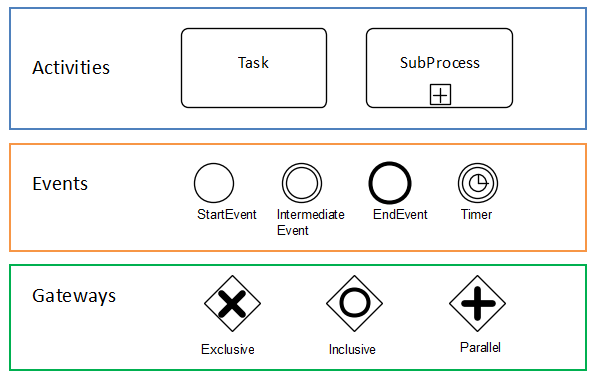
\includegraphics[width=.9\textwidth]{figuras/BPMNBasicSymbols.png}
%\caption{Principais elementos de um processo de acordo com o padrão BPMN. Fonte: NobleProg Training Materials}
%\label{fig:bpmn}
%\end{figure}

Uma \emph{Activiti} é a menor parte de um diagrama BPM, e é utilizada quando o diagrama não pode ser dividido mais detalhadamente. Quando uma \emph{Activiti} está inserida no contexto de um processo, ela é chamada de \emph{Task}. Geralmente as Tasks são executadas por um usuário final ou por uma aplicação. Existem diferentes tipos de Tasks para representar os diferentes comportamentos que cada tarefa pode representar. Por exemplo, uma \emph{userTask} representa uma tarefa em que um usuário deve executar uma ação.
%represent. The list of Task types MAY be extended along with any corresponding indicators. \emph{userTask},\emph{manualTask}.

%events
Um \emph{Event} é algo que "acontece" durante o curso de um processo\cite{model2011notation}. Existem três tipos principais de eventos: Start Event (indica o início do processo), End Event (indica um fim do processo) e Intermediate Events (indica um evento entre o início e o fim do processo).

%gateways
\emph{Gateways} são usados para controlar o fluxo do processo. Em gateways do tipo \emph{Exclusive}, apenas um dos caminhos que partem do gateway poderão ser seguidos, já em gateways do tipo \emph{Inclusive} um ou mais caminhos podem ser seguidos. Em gateways do tipo \emph{Parallel} todos os caminhos são tomados em paralelo.

%A Parallel Gateway is used to synchronize (combine) parallel flows and to create parallel flows.? The Parallel Gateway MUST use a marker that is in the shape of 
%plus sign and is placed within the Gateway
%diamond (see Figure 10.110) to distinguish it from other Gateway

%sequence flows
Um elemento \emph{Sequence Flow} é usado para exibir a ordem em que os demais elementos são executados em um processo. Cada \emph{sequenceFlow} possui um atributo \emph{sourceRef} que indica de onde este \emph{sequenceFlow} vem, ou sua "fonte", e um atributo \emph{targetRef} que indica para onde ele vai, ou seja, seu alvo. Cada \emph{sequenceFlow} possui apenas possui apenas uma fonte e um alvo. Analisando os elementos \emph{sequenceFlow} e analisando os dois atributos citados acima é possível identificar todo o fluxo do processo.


\section{Teste Funcional de Software}
O teste funcional é um tipo de teste que permite verificar as saídas de um sistema produzidas a partir de entradas pré-definidas. Este tipo de teste permite testar as funcionalidades, requerimentos e regras de negócio presentes no software\cite{molinari2003testes} verificando a existência de erros, o que auxilia na melhoria da qualidade do software.

Uma das principais medidas para o teste de software é a cobertura de teste. A cobertura de teste mede a abrangência do teste e pode ser expressa pela cobertura dos casos de testes ou pela cobertura do código executado. Existem diversos trabalhos que abordam a importância da cobertura de testes de software\cite{zhu1997software,bieman1996using}, inclusive ligando o crescimento da qualidade e confiabilidade do software ao crescimento da cobertura dos testes\cite{malaiya2002software}.
%Por esses motivos o aumento da cobertura dos testes de software também é um assunto bastante abordado\cite{}.

%Essa cobertura pode se basear em fluxos de controle (instrução, ramificação ou caminhos) ou fluxos de dados. Na cobertura baseada em fluxo de controle, o objetivo é %testar linhas de código, condições de ramificação, caminhos que percorrem o código ou outros elementos do fluxo de controle do software. Na cobertura baseada em fluxo %de dados, o objetivo é testar se os estados dos dados permanecem válidos durante a operação do software, por exemplo, se um elemento de dados é definido antes de ser %usado.

No entanto, as atividades executadas para criar testes funcionais com uma boa cobertura podem muitas vezes se tornar exaustivas e trabalhosas, dificultando assim a execução dos testes de forma adequada. Com o objetivo de melhorar a qualidade da análise e o tempo de execução dos testes, foram criados os testes automatizados, que proporcionam a execução dos testes mais rapidamente \cite{fantinato2005autotest}. Quando executada corretamente, a automação de teste é uma das melhores formas de reduzir o tempo de teste no ciclo de vida do software, diminuindo o custo e aumentando a produtividade do desenvolvimento de software como um todo, além de, consequentemente, aumentar a qualidade do produto final.

Para executar os testes funcionais automatizados em aplicações Web, pode-se utilizar ferramentas livres como Selenium\cite{selenium}, Watir\cite{watir} ou Geb\cite{geb}. No trabalho anterior\cite{sbqs2015}, onde os testes funcionais se mostraram mais promissores, foi utilizada a ferramenta Selenium, aliada ao Cucumber-JVM\cite{cucumber} para descrição dos testes. A escolha foi motivada pelo grande número de referências ao Selenium na Web, confirmadas por um trabalho que apresentou resultados satisfatórios com Selenium e Cucumber\cite{pannutest,sbqs2013}.

%Selenium is composed of multiple software tools. Each has a specific role.

%For this work, we picked up the Selenium tool that is an integrated development environment for automated test scripts, it is implemented as a Firefox extension, and allows to record, edit, and debug tests. Also, combined with Selenium, we picked up the Cucumber-JVM\footnote{Cucumber-JVM. Available at: www.github.com/cucumber/cucumber-jvm.} tool for a description of the tests, Cucumber is a tool that provides a high-level interface that allows to write tests in natural language.

\subsection{Teste Funcional Automatizado utilizando \emph{Selenium} e \emph{Cucumber-JVM}}
O processo para a execução de um teste funcional utilizando o Selenium aliado ao Cucumber-JVM é composto de cinco etapas: captura da interação do usuário com a aplicação e exportação do código gerado, criação dos cenários de teste, criação das definições dos passos de teste, implementação dos métodos para cada passo e, por fim, execução do teste.

Para efetuar a captura da interação do usuário com a aplicação é utilizado o Selenium IDE (\emph{Integrated Development Environment}), que permite gravar as ações do usuário conforme elas são executadas. Assim, a funcionalidade que deseja ser testada deve ser executada para que os passos sejam gravados. Após a captura da interação é possível exportar o \emph{script} utilizando diversas linguagens de programação disponíveis, neste caso foi escolhida a linguagem Java.

Os testes utilizando o Cucumber são compostos, basicamente, por dois arquivos: arquivos que especificam as funcionalidades \emph{features} e por arquivos de definição de passos \emph{steps}. 

Os arquivos com as funcionalidades são escritos utilizando a linguagem Gherkin\cite{gherkin} e são compostos por cenários, os cenários representam uma fração da aplicação que vai ser testada. Um cenário também pode ser descrito como a definição, em ordem de execução, das etapas que são executados nessa fração, bem como dos resultados esperados para validar a aplicação. Por exemplo, após um \emph{gateway} exclusivo com dois caminhos disponíveis, já é possível obter dois cenários possíves: um cenário executando cada caminho.
%Por exemplo, para testar apenas o login em uma aplicação, já é possível obter dois cenários possíveis: (a) dados de acessos corretos e sucesso no login e (b) dados de acesso incorretos e mensagem de erro. 

Para que cada etapa do cenário seja executada, é necessária a criação de \emph{steps} que irão traduzir os passos definidos na linguagem Gherkin para ações que vão interagir com o sistema. Cada \emph{step}, geralmente, irá chamar um método Java que irá efetivamente executar a interação com a aplicação. A implementação destes métodos pode ser feita apenas utilizando o código extraído através do Selenium após a captura das ações do usuário.

Assim, mesmo utilizando o Cucumber e Selenium para facilitar a criação dos testes, ainda é preciso analisar o processo e extrair os cenários de teste que devem ser criados manualmente no arquivo de \emph{features}. Além dos cenários, também deve ser criado manualmente o arquivo de \emph{steps}, contendo uma "passo" correspondente a cada etapa de todos os cenários criados. Esta etapa pode ser trabalhosa, principalmente quando for necessário testar todos diversos cenários que um processo pode ter ou quando o processo for extenso.

%When Cucumber executes a Step in a Scenario it will look for a matching Step Definition to execute.
%A Step Definition is a small piece of code with a pattern attached to it. The pattern is used to link the step definition to all the matching Steps, and the code is what Cucumber will execute when it sees a Gherkin Step.
%/Selenium 2 (aka. Selenium WebDriver)
%Selenium 2 is the future direction of the project and the newest addition to the Selenium toolkit. This brand new automation tool provides all sorts of awesome features, including a more cohesive and object oriented API as well as an answer to the limitations of the old implementation.
%Selenium 2.0 is the product of that effort. It supports the WebDriver API and underlying technology, along with the Selenium 1 technology underneath the WebDriver API for maximum flexibility in porting your tests. In addition, Selenium 2 still runs Selenium 1’s Selenium RC interface for backwards compatibility.
%cenário de BDD. Ou seja, descrevemos o que (comportamento) do sistema com cenários de critérios de aceite, mas quando vamos implementar seus detalhes e testar o como ele implementa essa funcionalidade, usamos TDD.
% \begin{itemize}
%   \item Como é feito o teste;
%   \item Explicação dos elementos principais do teste (cenários e stepDefinition);
%   \item Problema: Criação destes elementos pode ser trabalhoso (processos grandes com muitas tarefas ou com muitos caminhos possíveis).
% \end{itemize}

\section{BPMN Parser}
O objetivo deste trabalho é melhorar e facilitar o teste funcional automatizado de aplicações BPM. A criação dos cenários de teste utilizados pelo Cucumber é uma etapa importante para a melhoria do teste, pois estes podem definir ou limitar o que será testado, interferindo assim na qualidade e na cobertura dos testes. No entanto a criação dos arquivos de \emph{features} contendo os cenários e do arquivo de \emph{steps} pode ser trabalhosa, como foi mencionado na seção anterior.

Com o objetivo de facilitar a criação dos artefatos utilizados no teste funcional com o Cucumber-JVM, o arquivo de cenários e o arquivo de \emph{steps}, decidiu-se analisar os arquivos XML no formato BPMN exportados pelas ferramentas BPMS para extrair destes arquivos informações úteis. 

Para analisar os arquivos foi desenvolvido um \emph{parser} que percorre os arquivos XML e manipula as informações necessárias. O \emph{parser} foi criado utilizando a linguagem Java, principalmente por esta linguagem já possuir uma ferramenta sólida para a análise de documentos XML\cite{javadom}.  Os processos utilizados para a validação do parser foram obtidos no site da \emph{Object Management Group} (OMG) e estão disponíveis em \href{https://colocar link}{colocar link}. Basicamente, o \emph{parser} criado percorre o arquivo BPMN e analisa os elementos através da nomentaclatura padrão das \emph{tags} no arquivo e então executa uma lógica para criar os diferentes cenários de teste. Ao fim da execução são criados os arquivos de \emph{features} e \emph{steps} para o teste funcional. Juntamente com os arquivos para o teste, é gerado um arquivo Excel contendo uma tabela com os todos os possíveis cenários/caminhos do processo, facilitando a visualização do que será testado.

%\begin{itemize}
%\item Objetivo: gerar artefatos para melhoria do teste funcional automatizado de aplicações bpm; gerar arquivo de features e de steps;
%\item Informações técnicas (linguagem, etc) + onde foram obtidos os diagramas utilizados para validação;
%\item Resuminho do que ele faz: gera tabelinha + uma parte dos códigos
%\end{itemize}

%arquivo bpmn é exportado
%onde foram obtidos os diagramas que foram testados nesse trabalho
%The Object Management Group (OMG) has developed a standard Business Process Model and Notation (BPMN).
%The primary goal of BPMN is to provide a notation that is readily understandable by all business users, from the business
%analysts that create the initial drafts of the processes, to the technical developers responsible for implementing the
%technology that will perform those processes, and finally, to the business people who will manage and monitor those
%processes. Thus, BPMN creates a standardized bridge for the gap between the business process design and process
%implementation.

\subsection{Funcionamento do \emph{parser}}
%colocar uma citação pra array de adjacencias
O principal elemento para o funcionamento do parser é o \emph{Sequence Flow}. Por conter os atributos targetRef e sourceRef os elementos deste tipo permitem percorrer todo o diagrama. Ao iniciar o parser, é solicitado ao usuário o caminho para o arquivo BPMN e a ID do processo a ser avaliado. Um diagrama pode conter mais de um processo e, nesse caso, o usuário pode escolher que todos processos sejam avaliados.

A classe \emph{Node} define um tipo de objeto que guarda informações básicas sobre as tarefas do processo e um \emph{array} de objetos da mesma classe. Durante a execução do parser um array de objetos da classe Node é preenchido formando assim um array de adjacências. O método principal do parser percorre o processo recursivamente através dos elementos do tipo \emph{Sequence Flow}, enquanto um tarefa for encontrada, um objeto da classe Node é criado e o método é chamado recursivamente de modo a retornar o array de adjacências para este objeto.

A partir do array de adjacências são criados os caminhos possíveis pelos quais o processo pode passar. O método que cria os caminhos percorre recursivamente o array de adjacências criado anteriormente e "constrói" um novo caminho, tendo como condição de parada o encontro de uma das últimas tarefas a serem executadas. Uma tarefa é uma das últimas quando o elemento que a sucede no fluxo for \emph{End Event}. Ao encontrar uma tarefa final, o caminho é armazenado e é iniciada a construção de um novo caminho.

Os caminhos obtidos são base para a criação dos dois artefatos para o teste funcional: tabela de caminhos possíveis e código para o teste funcional. Para criar a tabela com os caminhos possíveis, cada tarefa existente no processo representará uma coluna na tabela e cada caminho representará uma nova linha. Para cada caminho, se a tarefa estiver presente a coluna será marcada com "X" caso contrário a coluna será marcada com um "0". Caso mais de um processo seja avaliado ao mesmo tempo, a tabela referente à cada processo estará separada individualmente no arquivo final. Na Tabela \ref{tab:exemplo}, pode ser visto uma tabela resultante da execução do parser para um processo com cinco \emph{tasks} e dois caminhos possíveis. 

Para a criação do código para o teste funcional dois arquivos devem ser criados: o arquivo contendo os cenários e a classe \emph{stepDefinition} contendo os métodos para cada passo do cenário. Para criar estes artefatos, cada caminho obtido é considerado um cenário diferente. Como trata-se de um teste funcional, apenas tarefas que podem ser executadas por um usuário devem ser avaliadas (\emph{userTask},\emph{manualTask}...). Assim, para cada caminho é criado um novo cenário utilizando a notação do Cucumber e comtemplando apenas as tarefas que podem ser executadas por um usuário. O método correspondente a cada passo do cenário é criado ao mesmo tempo. Na Figura \ref{fig:exemplo_cenario}, podem ser vistos dois cenários resultante da execução do parser para um processo com dois caminhos possíveis. 

\begin{figure}[ht]
\centering
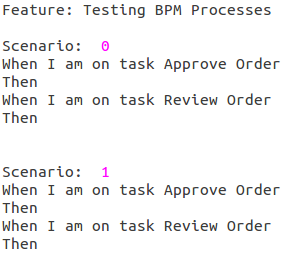
\includegraphics[width=.5\textwidth]{figuras/exemplo_cenario.png}
\caption{Exemplo de cenários resultantes}
\label{fig:exemplo_cenario}
\end{figure}

%explicar imagem, os arquivos conterão varios processos e varios métodos, ambos precisam ser completados para a execução do teste

\subsection{Dificuldades/Limitações}
Algumas ferramentas exportam o diagrama para o formato BPMN inserindo um ``tipo'' antes no nome de cada tag XML, por exemplo, a tag de nome task pode estar representada como ``semantic:task'' e isso pode impedir que o parser do Java identifique os elementos. Assim, foi necessário preparar o parser para tratar este tipo de situação.

\begin{table}[]
\centering
\caption{Exemplo de tabela resultante}
\label{tab:exemplo}
\begin{tabular}{ccccc}
\multicolumn{1}{l}{Quotation Handling} & \multicolumn{1}{l}{Approve Order} & \multicolumn{1}{l}{Order Handling} & \multicolumn{1}{l}{Shipping Handling} & \multicolumn{1}{l}{Review Order} \\
X & X & 0 & 0 & 0 \\
X & X & X & X & X
\end{tabular}
\end{table}


Na criação dos artefatos para o teste funcional são levados em conta apenas tarefas que podem ser executadas por um usuário. Apesar de utilizarem o mesmo padrão BPMN, algumas ferramentas podem utilizar nomes diferentes parat representar estas tarefas no arquivo XML. Por isso, dependendo da tarefa que for utilizada, pode ser necessário substituir o nome dos tipos a serem utilizados no parser.

%pode gerar caminhos iguais, por remover boa parte das tarefas, como pdoe ser visto na figura de antes também

%-subprocess -> apenas como uma tarefa, normalmente sao simples, so testa o principal,subprocessos normalmente sao simples

Na criação dos caminhos, uma dificuldade ocorreu devido aos desvios causados por elementos do tipo \emph{Gateway}. Para isso, para cada Node criado no array é guardada o tipo do elemento que o antecede. Assim, na criação dos caminhos, elementos que partem de um desvio de fluxo precisaram ser tratados para criar os caminhos corretamente, por exemplo: se dois elementos, X e Y, vem de um gateway exclusivo, os caminhos obtidos até estes elementos serão duplicados, ou seja, metade dos caminhos passaram apenas por X e metade dos caminhos passarão apenas por Y.

%Na criação dos caminhos, há uma exceção para quando existir uma divisão de fluxo através de um gateway do tipo inclusivo. Diferente do que acontece com o tipo exclusivo, onde apenas uma opção de pode ser seguida de cada vez, no caminho incluso as opções podem variar pois um ou mais caminhos podem ser seguidos ao mesmo tempo. Os caminhos em que apenas um fluxo é seguido já são cobertos pela execução normal do parser, então, após a criação dos caminhos, é identificada a existencia de fluxos inclusivos e, se necessário, caminhos adicionais são inseridos.

Devido ao fato de o parser ser executado recursivamente e percorrer o processo baseado no fluxo dos elementos do tipo \emph{sequenceFlow}, ocorreram problemas em processos onde uma parcela do processo também é executada recursivamente. Estes problemas foram causados devido ao fluxo nunca encontrar um "fim". Para solucionar esses problema foi criado um "delimitador de recursão" que define e controla o número de vezes em que o mesmo \emph{sequenceFlow} será executado.


%o cenário contem qual tarefa vai ser executada e em que ordem, mais algumas etapas ainda precisam ser preenchidas
%alguns caminhos podem se repetir pois apenas tarefas executadas por usuario são levadas em conta, poderia faz pra não tratar essas tarefas

%anotações anteriores
%Após isso, é iniciada a avaliação de cada processo. O parser percorre os elementos do tipo sequenceFlow em busca das primeiras tarefas do processo, ou seja, tarefas que sucedem elementos do tipo startEvent. Para cada tarefa encontrada, será criado um objeto da classe definida como “Node” que contém informações básicas sobre os elementos e mais um array de adjacência. 
%Então é feita a criação dos arrays de adjacência. No método chamado createNodes que retorna um objeto do tipo List<Node>, são percorridos todos os elementos sequenceFlow partindo das primeiras tarefas e, para cada nova tarefa encontrada, é criado um objeto da classe Node e então o método é chamado recursivamente para obter o array de adjacência do elemento em questão. O trecho de código referente a essa execução pode ser visto na Figura X. Este método é executado recursivamente até encontrar um elemento do tipo endEvent, ou seja, até encontrar um fim.
%Assim, têm-se uma lista de objetos da classe Node. Os primeiros elementos desta lista serão, obrigatóriamente, as primeiras tarefas que foram encontradas no início da execução. Estes elementos teram as informações pertinentes mais o array de ajacências, que também é uma lista de objetos Node. Nesta lista estarão contidos todos os objetos da classe Node que sucedem a tarefa anterior.
%Após o documento XML ser devidamente analisado e as tarefas do processo esterem armazenadas no array de objetos Node, é possível criar os artefatos para auxiliar no teste funcional. Uma parte importante para esta etapa é identificar as últimas tarefas à serem executadas, ou seja, tarefas que antecedem um elemento do tipo endEvent. %Estas tarefas irão auxiliar na criação dos possíveis caminhos pelos quais o processo pode passar.
%Para criar os possíveis caminhos do processo, o array de adjacências obtido anteriormente é navegado recursivamente até encontrar uma condição de parada: a(s) últimos tarefas a serem executadas. Para cada chamada deste método, é recebido o array e os elementos pelos quais esse caminho passou anteriomente, ao encontrar a condição de parada, este novo caminho é armazenado e é iniciado um novo caminho. %método paths
%A partir da criação dos caminhos, é chamado o método fillTable que percorre os caminhos para criar a tabela com os caminhos possíveis. No cabeçalho da tabela estarão presentes os nomes de todas as tarefas do processo e cada linha representa um caminho possível. O método fillTable ira percorrer todos os caminhos, comparando cada elemento do caminho com um elemento do processo, se o elemento faz parte deste caminho a coluna será marcada com um "X" caso contrário, a coluna será marcada com um "0". Ao final de toda a execução, a tabela será salva em um arquivo do tipo excel. Caso exista mais de um processo a ser analisado, as tabelas para cada processo estarão distribuídas individualmente no arquivo excel.


\section{Resultados}
Com a análise do arquivo BPMN através do parser criado foi possível obter dois arquivos essenciais para o teste funcional automatizado utilizando o Selenium e o Cucumber-JVM: o arquivo de \emph{features} contendo os cenários e o arquivo de \emph{steps} contendo métodos que para efetuar a execução de cada etapa do cenário. 

\begin{figure}[ht]
%\centering
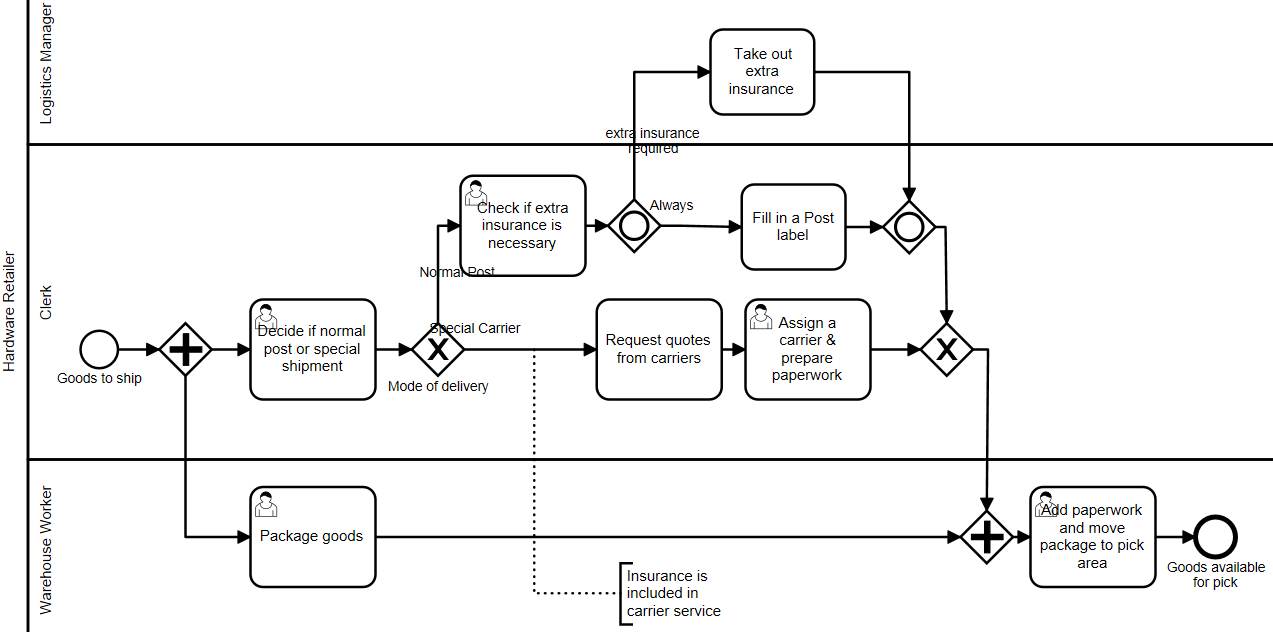
\includegraphics[width=.8\paperwidth]{figuras/diagrama_exemplo.png}
\caption{Exemplo de Processo. Adaptado de: Object Management Group}
\label{fig:diagrama_exemplo}
\end{figure}

Por exemplo, o processo na Figura \ref{fig:diagrama_exemplo} possui \emph{gateways} de diferentes tipos, gerando assim várias divisões de fluxo e aumentando os caminhos que podem ser seguidos. Para executar o teste completo do processo, testando todas as possibilidades e com boa cobertura, seria necessário planejar os cenários de teste e criá-los manualmente. Para criar os cenários também é necessário identificar quais tarefas são executadas por um usuário e o processo possui várias \emph{tasks}. Por fim, também seria necessário criar os \emph{steps} para cada etapa do cenário manualmente.

\begin{figure}[ht]
%\centering
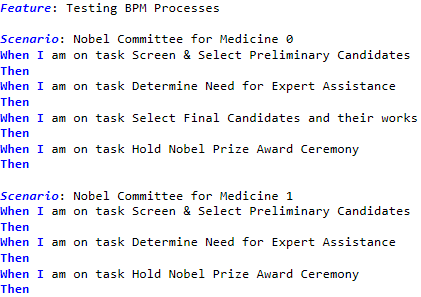
\includegraphics[width=.8\paperwidth]{figuras/cenario_resultado.png}
\caption{Cenários obtidos através do arquivo BPMN}
\label{fig:cenario_resultado}
\end{figure}

Executando o parser criado utilizando o arquivo BPMN referente ao diagrama da Figura \ref{fig:diagrama_exemplo} como exemplo, obtemos os cenários de teste representados na Figura \ref{fig:cenario_resultado}. Para o teste funcional do processo, três cenários são possíveis, representando as duas principais divisões de fluxo encontradas no processo. A primeira divisão de fluxo formada pelo \emph{gateway} do tipo paralelo logo no início do processo, está contida no cenário de forma que os cenários \emph{Hardware Retailer 0} e \emph{Hardware Retailer 1} fazem parte de um fluxo e o cenário \emph{Hardware Retailer 2} representa o segundo fluxo possível. A segunda divisão de fluxo no processo da Figura \ref{fig:diagrama_exemplo} é formada pelo \emph{gateway} do tipo exclusivo, e essa divisão é representada pelos cenários \emph{Hardware Retailer 0} e \emph{Hardware Retailer 1}. Há ainda uma terceira divisão de fluxo no processo, esta divisão não foi levada em conta pelo parser pois as tarefas subsequentes a essa divisão não são tarefas executadas pelo usuário.

Como foi mencionado anteriormente, apenas tarefas executadas por usuários são levadas em conta para o teste funcional, e por isso nem todas as tarefas do processo estarão presentes nos cenários de teste.

%o cenário contem qual tarefa vai ser executada e em que ordem, mais algumas etapas ainda precisam ser preenchidas

Para cada etapa nos cenários criados será criado um método correspondente dentro do arquivo de \emph{steps} chamado \emph{stepDefinition}. Uma parte do arquivo de \emph{steps} resultante da análise do processo em questão pode ser vista na Figura \ref{fig:steps_resultado}. Como pode ser visto nesta figura, para a etapa \emph{I am on the task Decide if normal post or special shipment} foi criado um método com um nome genérico e contendo a anotação \emph{@Given("\^{}I am on the task Decide if normal post or special shipment\textdollar{}") 
}. Os métodos podem ser preenchidos posteriormente com os dados gravados pelo Selenium na etapa de captura da interação com a aplicação.

%preencher e colocar imagem do step definition
\begin{figure}[ht]
%\centering
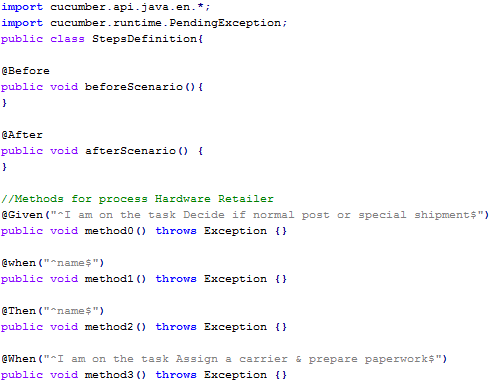
\includegraphics[width=.8\paperwidth]{figuras/steps.png}
\caption{Métodos obtidos através do arquivo BPMN}
\label{fig:steps_resultado}
\end{figure}

Neste exemplo, apenas um processo foi analisado, mas arquivos BPMN podem conter vários processos. Neste caso, se for necessário gerar os dados para todos os processos dentro de um arquivo, os arquivos de \emph{features} e \emph{steps} conterão, respectivamente, os cenários e métodos para todos os processos dentro do arquivo BPMN.


%\begin{itemize}
%\item Exemplo de processo, Figura \ref{fig:diagrama_exemplo};
%item Exemplo dos artefatos obtidos: tabelinha e cenário de teste (apenas necessário completar com os códigos obtidos no selenium)
%	\item Melhoria na criação dos testes (mais rápido e mais completo);
%	\item Por consequência: Melhoria na cobertura dos testes (todos caminhos e cenários possíveis)
%	\item Por consequência: auxilia na melhora da qualidade dos sistemas.
%\end{itemize}

Com estes resultados se dizer que este trabalho atingiu seu objetivo, pois foi possível obter dois arquivos muito importantes para a execução do teste funcional automatizado: o arquivo com os cenários de teste e o arquivo com os métodos para executar cada etapa dos cenários. A criação automatizada dos dois arquivos permite facilitar e melhorar a criação dos testes para os sistemas BPM, diminuindo o tempo de análise dos processos bem como tornando o teste mais completo ao mesmo tempo em que verifica todos os possíveis fluxos que um processo pode seguir. Assim, a qualidade e a cobertura dos testes também é melhorada pois todos os caminhos e cenários possíveis com tarefas executadas por usuários são criados. Por consequencia, a qualidade dos sistemas também pode ser beneficiada com um processo de teste mais completo e facilitado.

\section{Conclusão}
\begin{itemize}
\item Mesmo utilizando ferramentas para teste automatizado, criação dos elementos do teste podem ser trabalhosas;
\begin{itemize}
\item O parser criado auxilia nesse ponto.
\end{itemize}
\item Importante ter uma boa cobertura;
\item BPMN parser analiza a notação para gerar elementos para teste automatizado = facilita o teste e aumenta a cobertura.
\item Trabalhos futuros (tirar repeticoes de cenários, tentar gerar mais coisas,..)
\end{itemize}

\section{Referências}

\bibliographystyle{sbc}
\bibliography{sbc-template}

\end{document}
